%!TEX root = Slic3r-Manual.tex

\section{Cooling} % (fold)
\label{sec:cooling}
\index{cooling}
\index{temperature}

Temperature plays a key part in determining print quality.  Too hot and the material deforms, too cool and layer adhesion may be problematic.  Applying cooling will allow the freshly deposited material to solidify enough to provide a good base for the next layer, helping with overhangs, small details and bridges.

There are two main techniques for cooling: adding a fan and slowing down the print speed.  Slic3r may choose to use both techniques, using a fan first, and then slowing down the print if the layer time is too fast.

\begin{figure}[H]
\centering
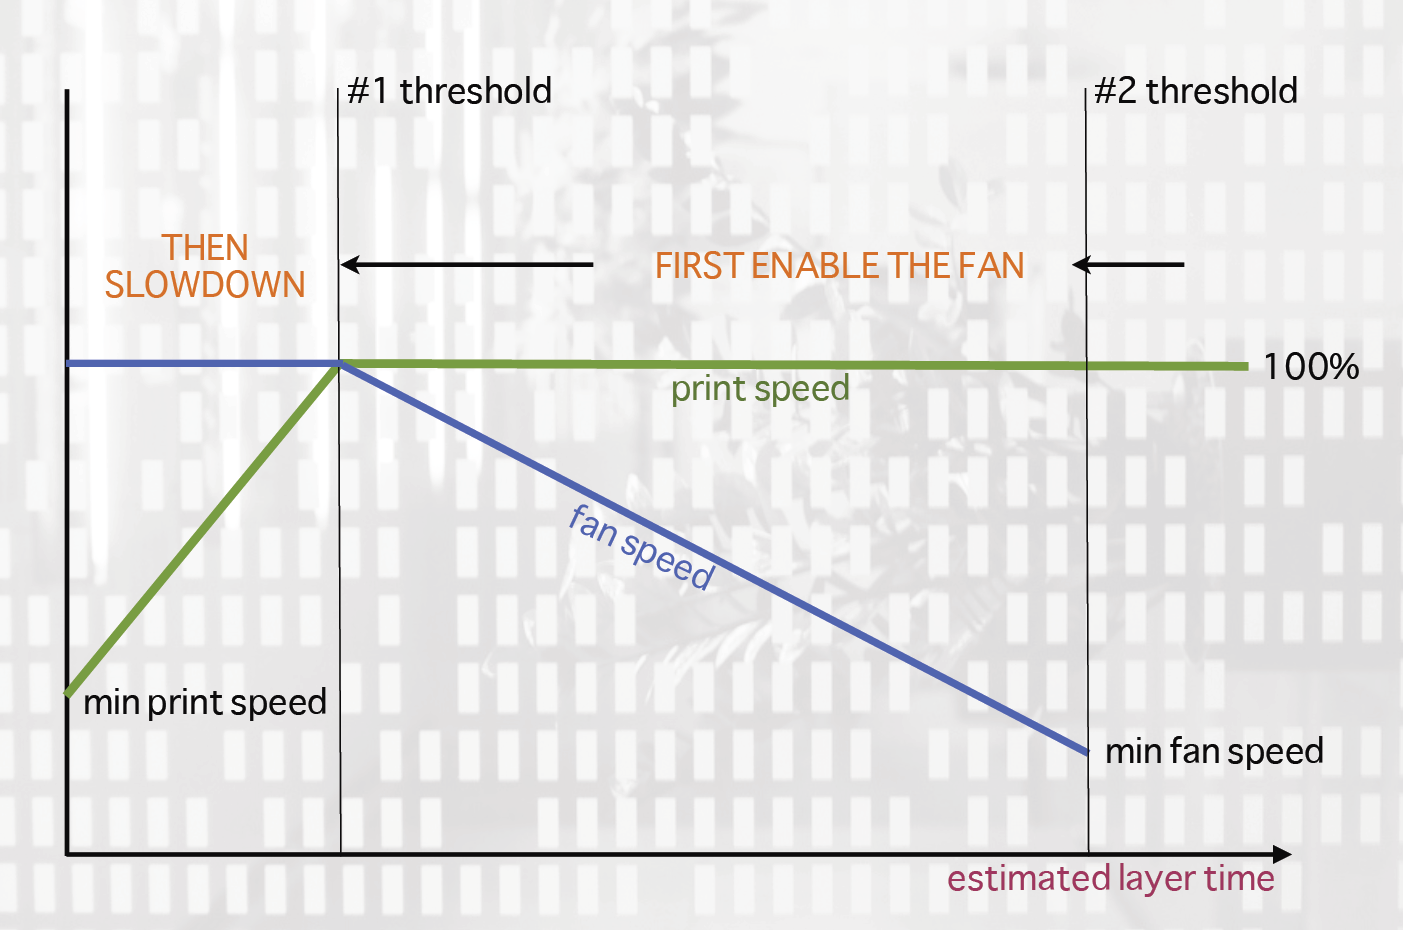
\includegraphics[keepaspectratio=true,width=1\textwidth]{expertmode/cooling_chart.png}
\caption{Cooling strategy.}
\label{fig:cooling_chart}
\end{figure}

Figure \ref{fig:cooling_chart} shows the strategy adopted by Slic3r.  Reading from right to left, when the minimum fan threshold (\#2) is reached the fan is turned on.  This increases in intensity as the layer time decreases.  The print speed remains constant until the estimated print time drops below a certain threshold (\#1), this is when the print speed is reduced until it reaches it's minimum value.

\subsection{Fans} % (fold)
\label{sub:fans}
\index{cooling!fans}
Most electronics and firmware allow the addition of a fan via a spare connector.  These can then be instructed with G-code, from Slic3r, to turn on or off as the model requires, and to rotate at different speeds.

Care should be taken with the positioning of the fan so that it does not cool any heated bed more than necessary.  It should also not cool the heater block of the hot-end so as not to force it to do more work and waste energy.  The air movement should aim for the nozzle tip, flowing over the freshly extruded material.

A duct may help in guiding the flow correctly, and there are several designs available online, for a wide variety of printers.

% subsection fans (end)

\subsection{Slowing Down} % (fold)
\label{sub:slowing_down}
\index{cooling!slowing down}
Slic3r can tell the printer to slow down if the estimated layer time is above a certain threshold.

Care must be taken as the intended effect could be mitigated by the nozzle not moving far enough away from the fresh extrusion, a problem with small, detailed layers.  For this reason it is usually recommended to use a fan where possible.
% subsection slowing_down (end)

\subsection{Configuring} % (fold)
\label{sub:configuring_cooling}

In simple mode Slic3r will attempt to choose the optimal settings for both fans and speed.  Expert mode gives more granular options.

\begin{figure}[H]
\centering
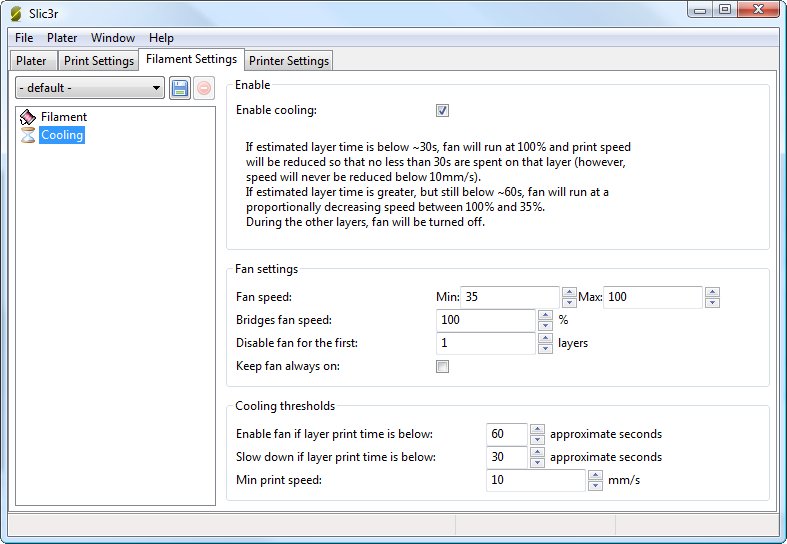
\includegraphics[keepaspectratio=true,width=1\textwidth]{expertmode/cooling_advanced_settings.png}
\caption{Cooling advanced settings.}
\label{fig:cooling_advanced_settings}
\end{figure}

\begin{itemize}
	\item \texttt{Fan speed}  - Determines the minimum and maximum speeds - useful for fans that run too fast by default.
	\item \texttt{Bridges fan speed}  - As the material stretches over wide gaps, it makes sense to try and cool it as much as possible, therefore a full fan speed is recommended.
	\item \texttt{Disable fan for first \textit{x} layers}  - Section \ref{sec:the_important_first_layer} detailed how important the first layer is, and so it makes sense not to apply the fan until sure the print is securely attached to the bed.  Keeping the fan turned off for the first two or three layers is a good idea.
	\item \texttt{Keep fan always on}  - Overrides any other choices and has the fan run continuously, at least at the minimum speed setting.  This can be useful when printing with PLA, but is not recommended for ABS.
\end{itemize}

\begin{itemize}
	\item \texttt{Enable fan if print time is below \textit{t} seconds}  - Triggers the fan if the layer will be completed within the given number of seconds.
	\item \texttt{Slow down if layer print time is below \textit{t} seconds}  - Slows down the print if the layer will be completed within the given number of seconds.
	\item \texttt{Min print speed}  - A lower limit on how slowly a layer can be printed.
\end{itemize}


% subsection configuring_cooling (end)

% section cooling (end)